\chapter{NAT (Static): Part 1}\label{nat-static-part-1}

PRIVATE IPv4 ADDRESSES (RFC 1918)

\begin{itemize}
\item
  IPv4 doesn't provide enough ADDRESSES for all DEVICES that need an IP
  ADDRESS in the modern world
\item
  The long-term solution is to switch to IPv6
\item
  There are THREE MAIN short-term solutions:

  \begin{itemize}
  \tightlist
  \item
    CIDR
  \item
    PRIVATE IPv4 ADDRESS
  \item
    NAT
  \end{itemize}
\item
  RFC 1918 specifies the following IPv4 ADDRESS RANGES as PRIVATE:

\begin{lstlisting}
10.0.0.0 /8       (10.0.0.0 to 10.255.255.255)             CLASS A
172.16.0.0 /12    (172.16.0.0 to 172.31.255.255)           CLASS B
192.168.0.0 /16   (192.168.0.0 to 192.168.255.255)         CLASS C
\end{lstlisting}
\item
  You are free to use these ADDRESSES in your NETWORKS. They don't have
  to be GLOBALLY UNIQUE
\end{itemize}

\begin{figure}
\centering
\pandocbounded{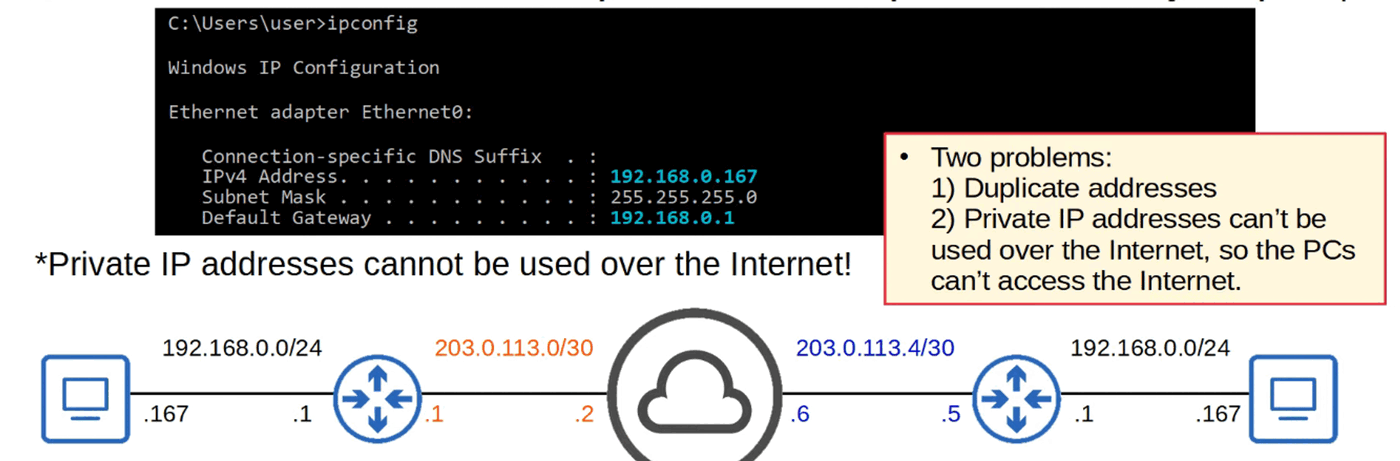
\includegraphics[keepaspectratio,alt={image}]{images/45-nat-static-part1/img-001.png}}
\end{figure}

\section{Intro to NAT}\label{intro-to-nat}

\begin{itemize}
\tightlist
\item
  NETWORK ADDRESS TRANSLATION (NAT) is used to modify the SOURCE and /
  or DESTINATION IP ADDRESSES of packets
\item
  There are various reasons to use NAT, but the MOST common reason is to
  ALLOW HOSTS with PRIVATE IP ADDRESSES to communicate with other HOSTS
  over the INTERNET
\item
  For the CCNA you have to understand SOURCE NAT and how to configure it
  on CISCO ROUTERS
\end{itemize}

\begin{figure}
\centering
\pandocbounded{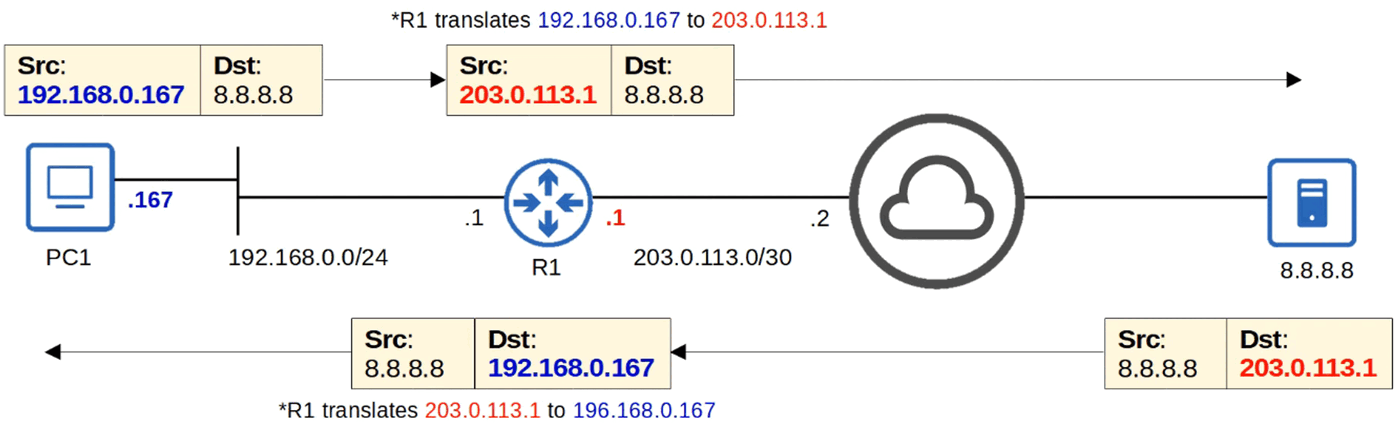
\includegraphics[keepaspectratio,alt={image}]{images/45-nat-static-part1/img-002.png}}
\end{figure}

\section{Static NAT}\label{static-nat}

\begin{itemize}
\tightlist
\item
  STATIC NAT involves statically configuring ONE-TO-ONE MAPPINGS of
  PRIVATE IP ADDRESSES to PUBLIC ADDRESSES
\end{itemize}

\begin{figure}
\centering
\pandocbounded{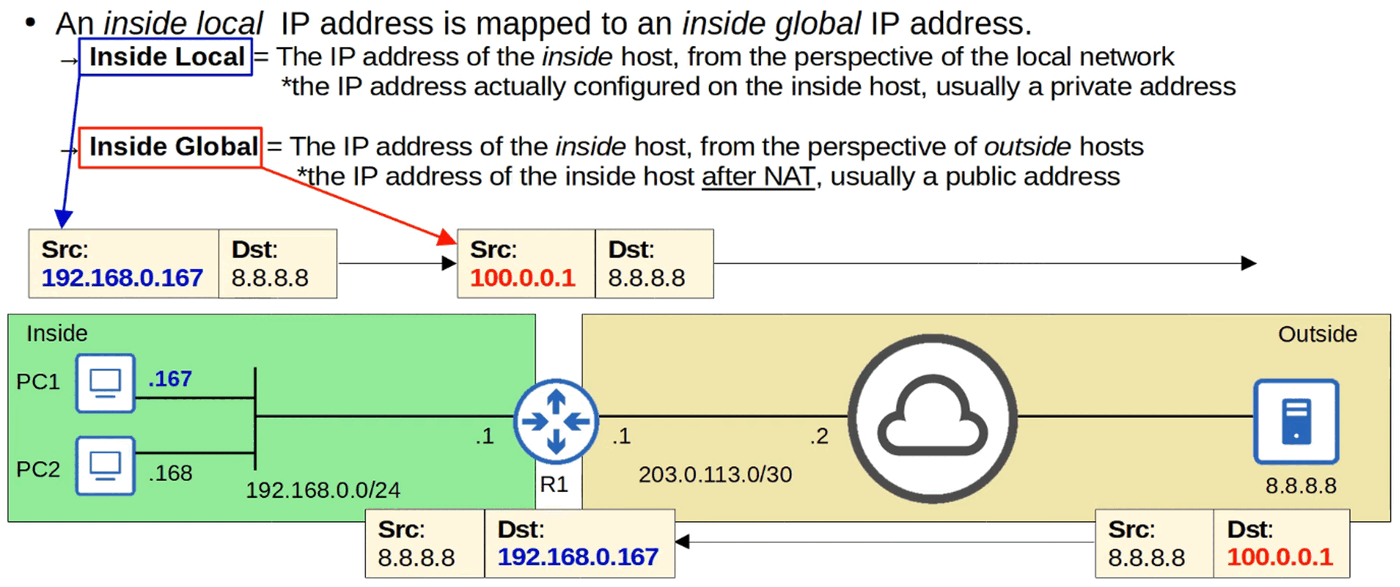
\includegraphics[keepaspectratio,alt={image}]{images/45-nat-static-part1/img-003.png}}
\end{figure}

\begin{figure}
\centering
\pandocbounded{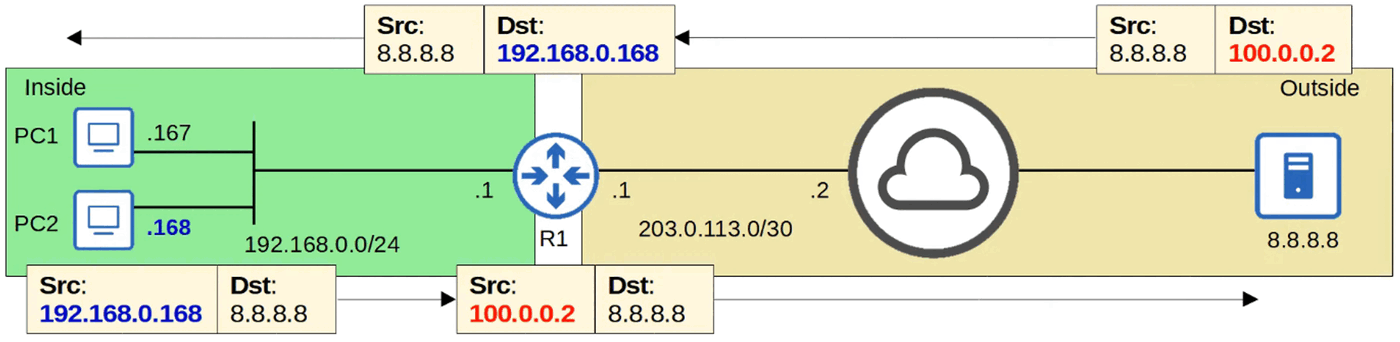
\includegraphics[keepaspectratio,alt={image}]{images/45-nat-static-part1/img-004.png}}
\end{figure}

\begin{figure}
\centering
\pandocbounded{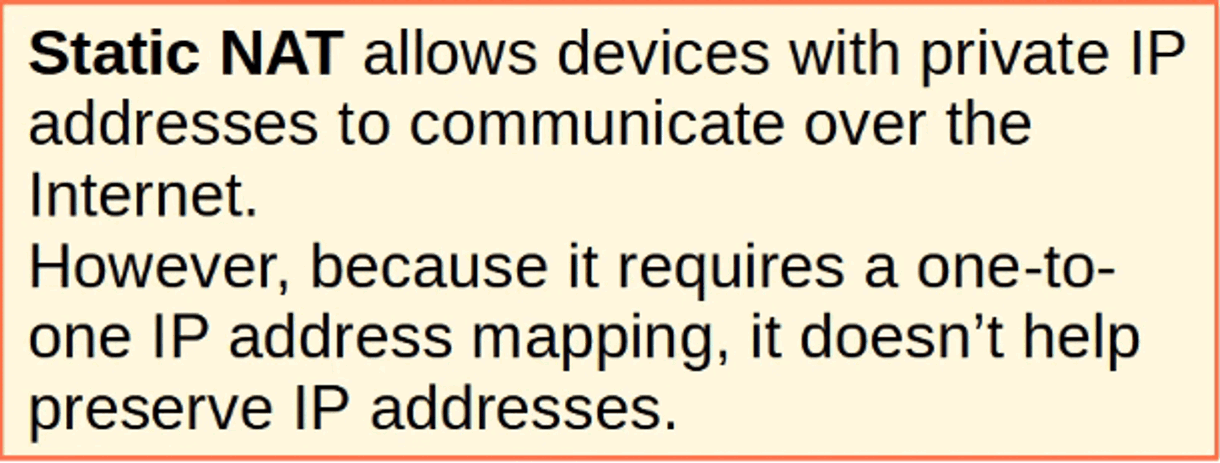
\includegraphics[keepaspectratio,alt={image}]{images/45-nat-static-part1/img-005.png}}
\end{figure}

\section{Private IP Cannot Be Mapped to the Same Global
IP}\label{private-ip-cannot-be-mapped-to-the-same-global-ip}

\section{The Second Mapping Will Be
Rejected}\label{the-second-mapping-will-be-rejected}

\begin{figure}
\centering
\pandocbounded{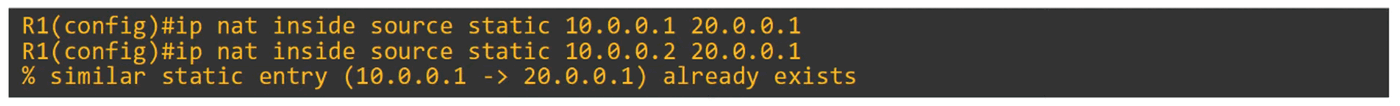
\includegraphics[keepaspectratio,alt={image}]{images/45-nat-static-part1/img-006.png}}
\end{figure}

\section{Static NAT Configurations}\label{static-nat-configurations}

\begin{figure}
\centering
\pandocbounded{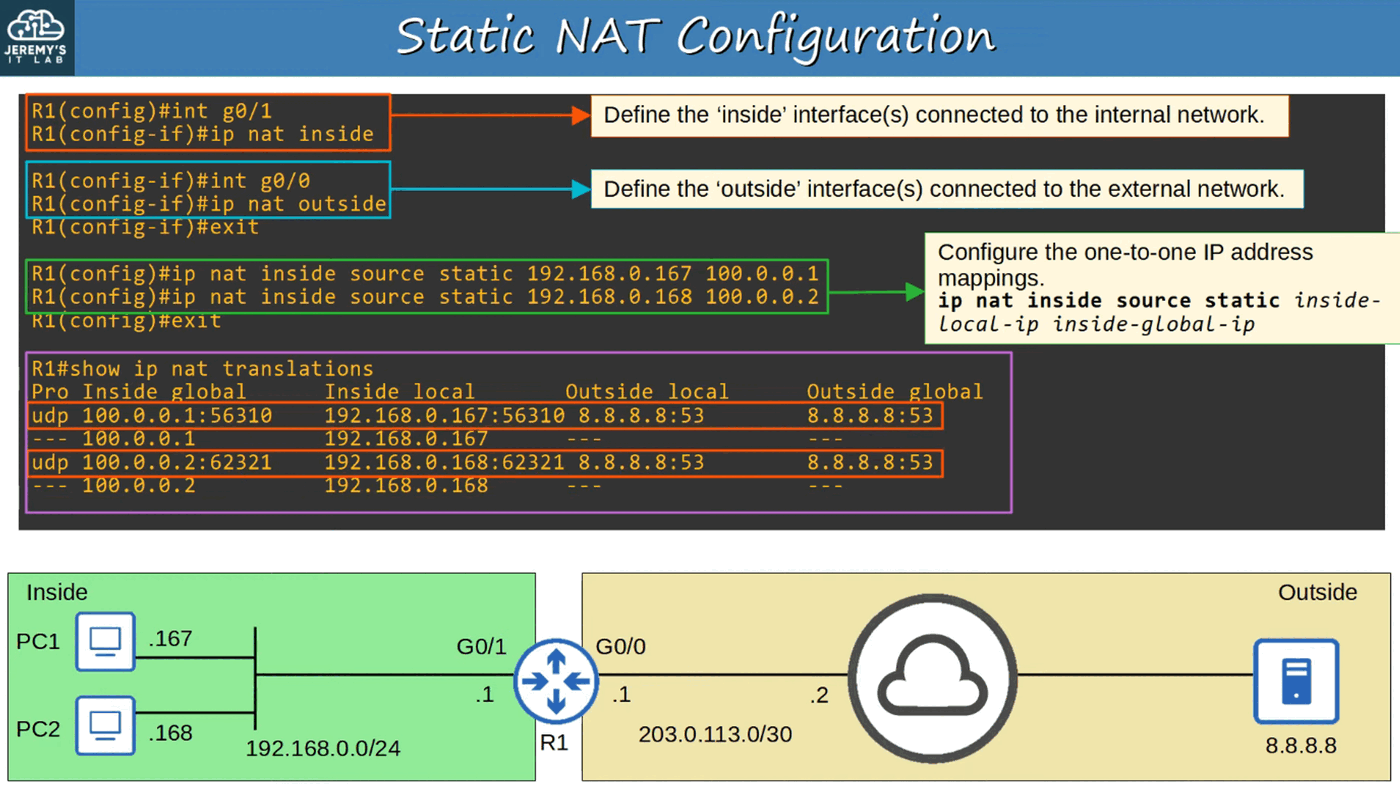
\includegraphics[keepaspectratio,alt={image}]{images/45-nat-static-part1/img-007.png}}
\end{figure}

\begin{figure}
\centering
\pandocbounded{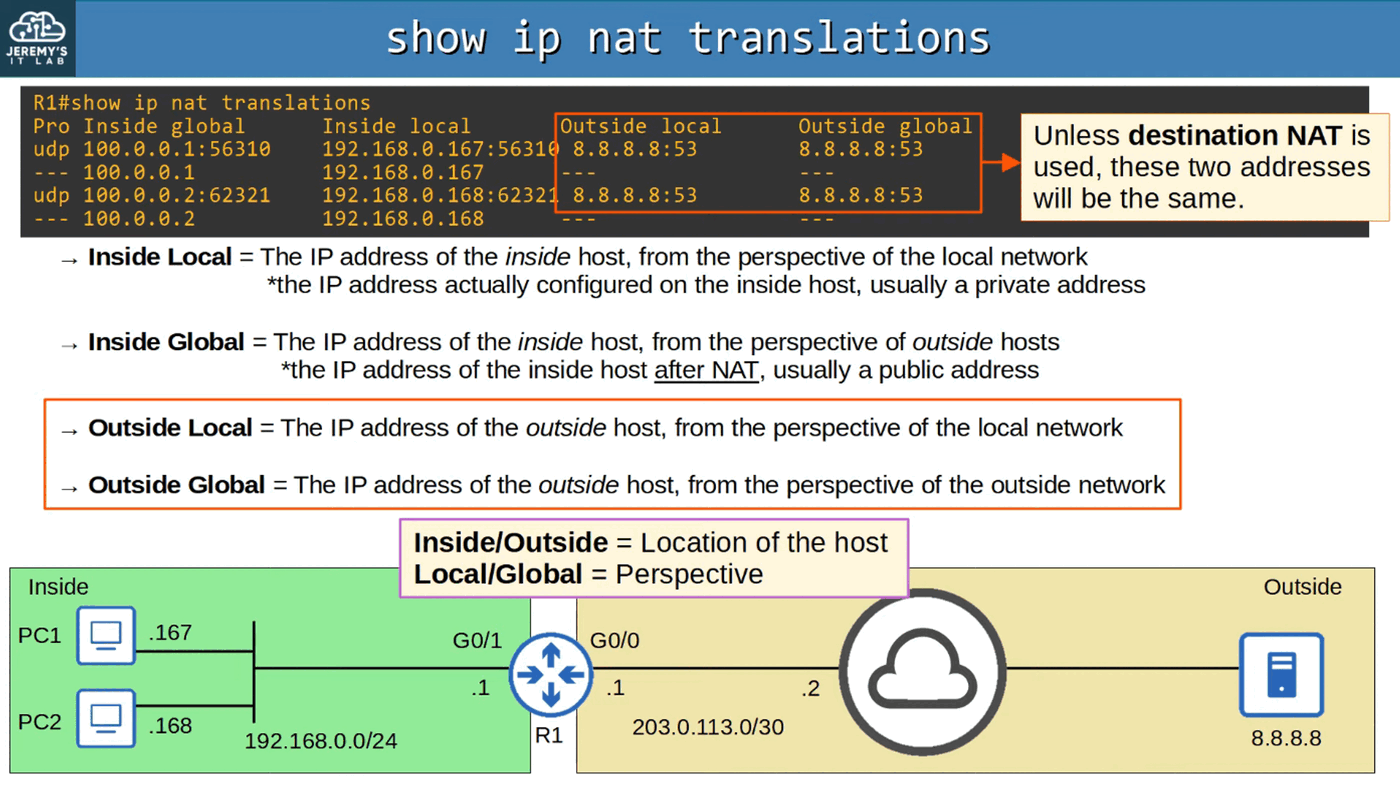
\includegraphics[keepaspectratio,alt={image}]{images/45-nat-static-part1/img-008.png}}
\end{figure}

Command \passthrough{\lstinline!clear ip nat translation!}

\begin{figure}
\centering
\pandocbounded{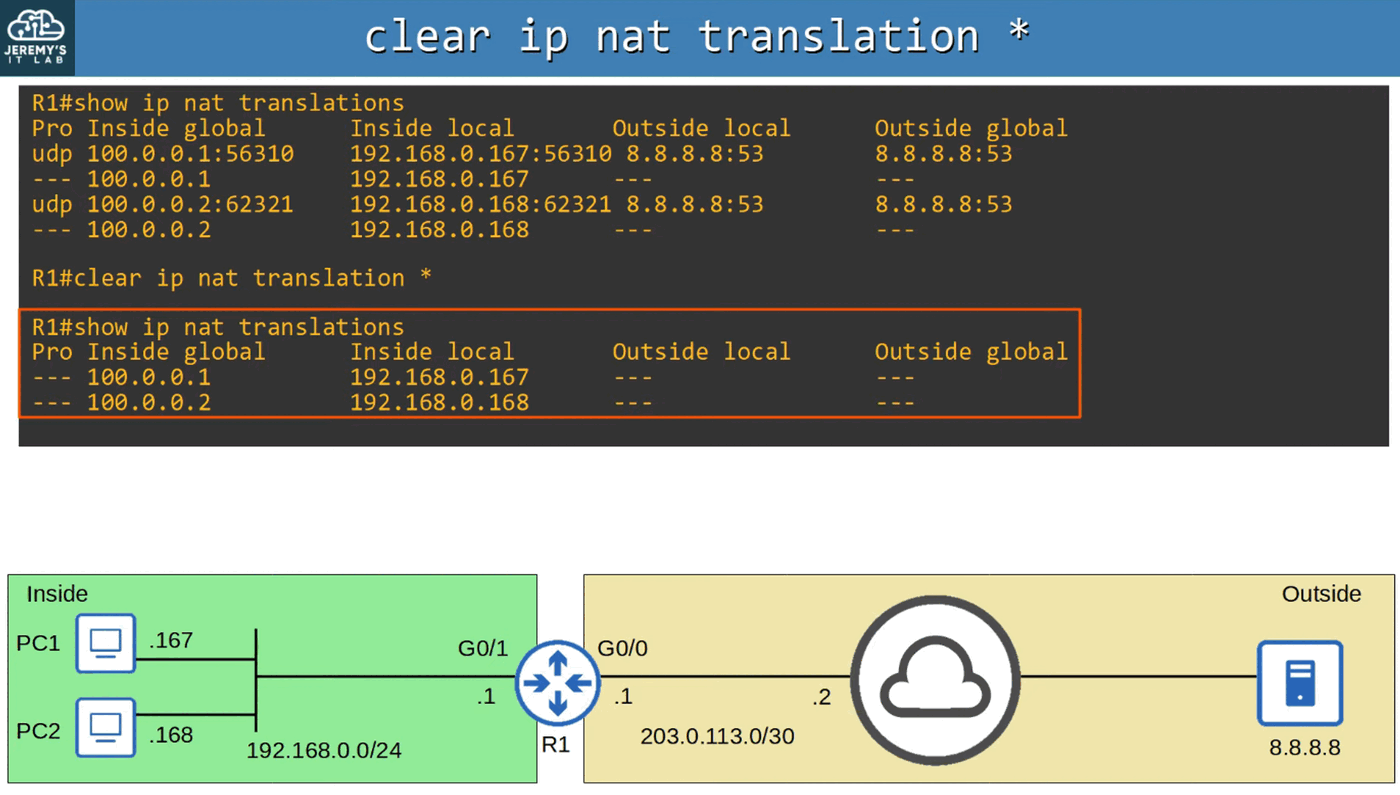
\includegraphics[keepaspectratio,alt={image}]{images/45-nat-static-part1/img-009.png}}
\end{figure}

Command \passthrough{\lstinline!show ip nat statistics!}

\begin{figure}
\centering
\pandocbounded{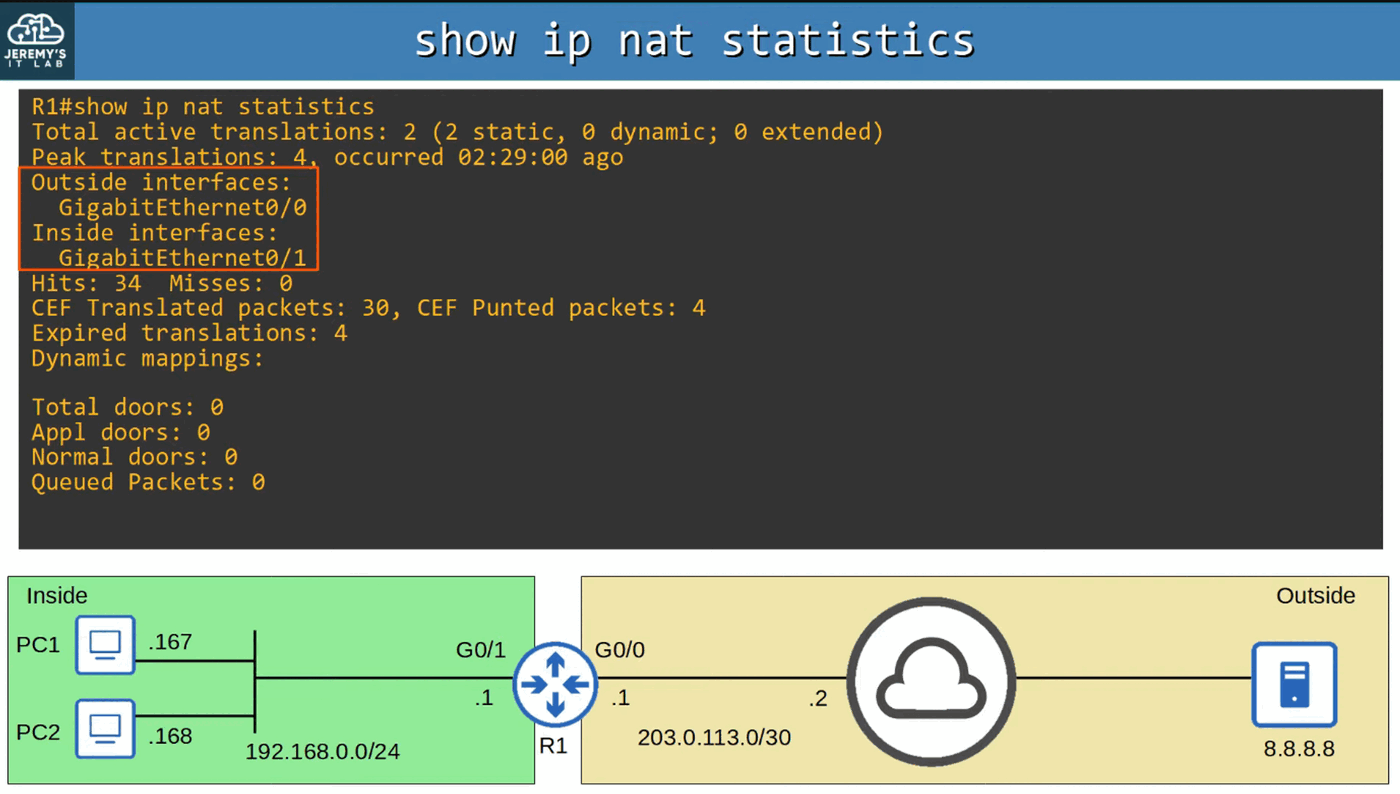
\includegraphics[keepaspectratio,alt={image}]{images/45-nat-static-part1/img-010.png}}
\end{figure}

\section{Command Review}\label{command-review}

\begin{figure}
\centering
\pandocbounded{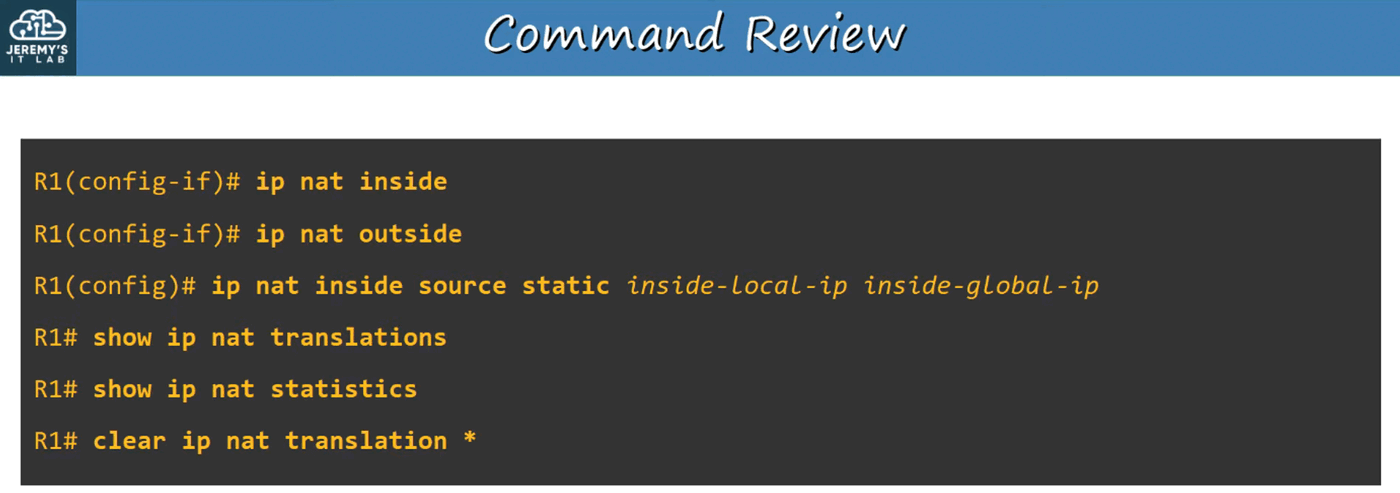
\includegraphics[keepaspectratio,alt={image}]{images/45-nat-static-part1/img-011.png}}
\end{figure}
